\chapter{Comparación entre distintas implementaciones}

\begin{figure}[H]
	\centering
	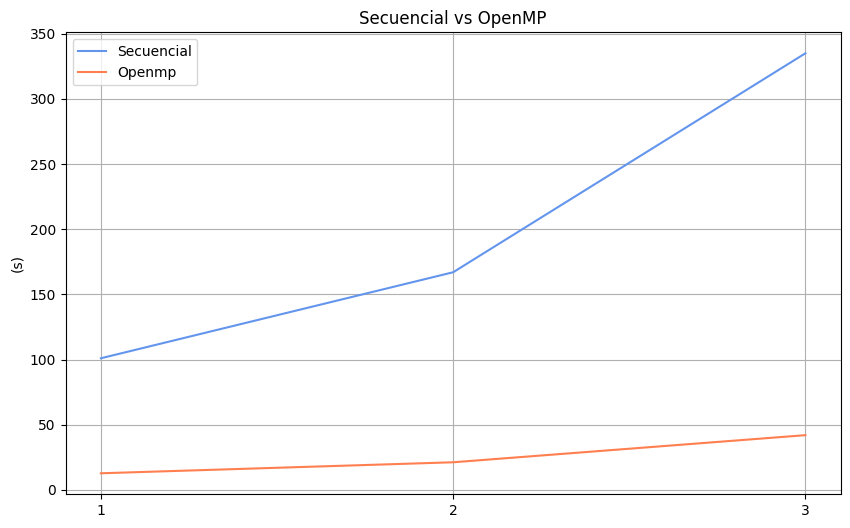
\includegraphics[scale=0.5]{imagenes/sec_openmp.png}  
	\caption{Secuencial vs OpenMP}
	\label{fig:sec_openmp}
\end{figure}

\begin{figure}[H]
	\centering
	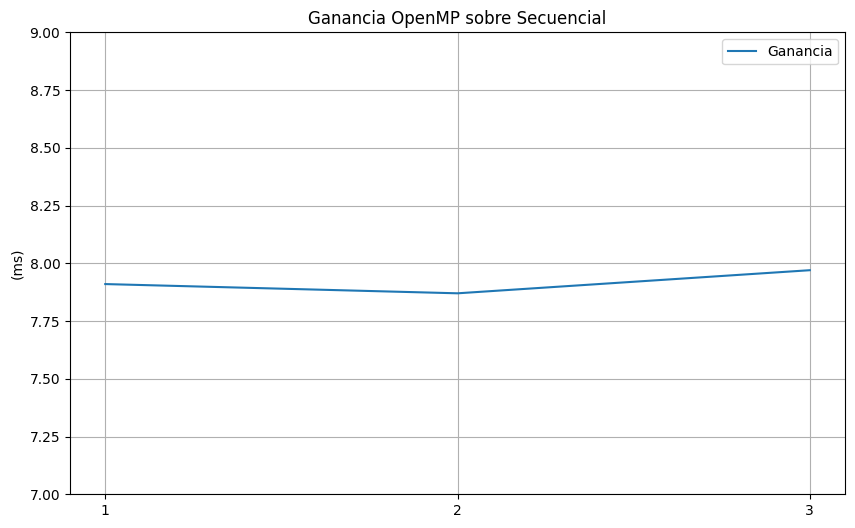
\includegraphics[scale=0.5]{imagenes/ganancia_sec_openmp.png}  
	\caption{Ganancia de OpenMP respecto a secuencial}
	\label{fig:ganancia_sec_openmp}
\end{figure}

\begin{figure}[H]
	\centering
	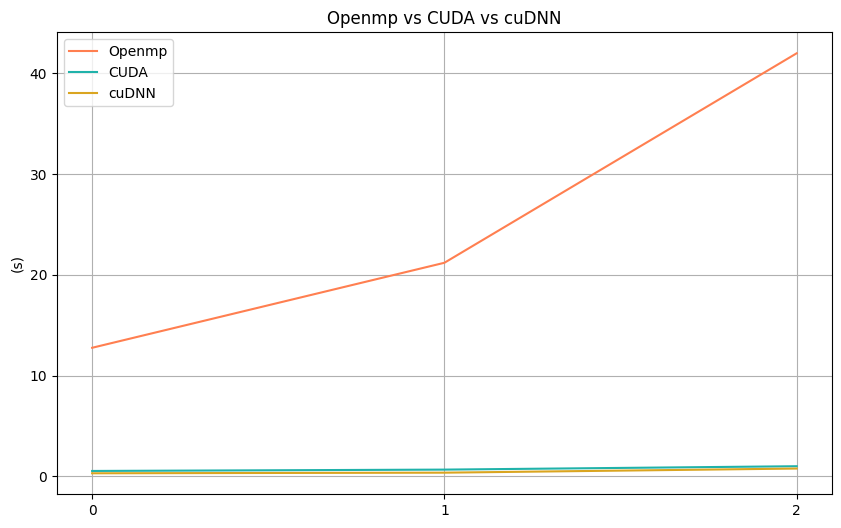
\includegraphics[scale=0.5]{imagenes/openmp_cuda_cudnn.png}  
	\caption{OpenMP vs CUDA vs CUDNN}
	\label{fig:openmp_cuda_cudnn}
\end{figure}

\begin{figure}[H]
	\centering
	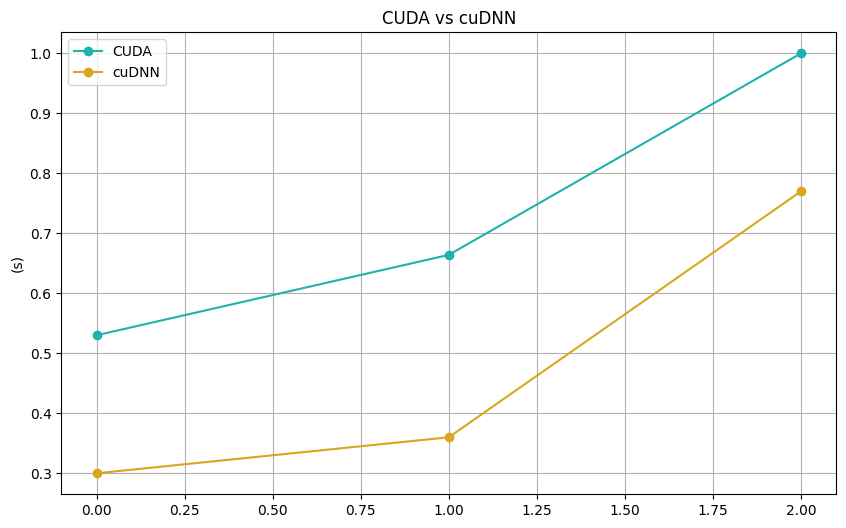
\includegraphics[scale=0.5]{imagenes/cuda_cudnn_1.png}  
	\caption{CUDA vs CUDNN}
	\label{fig:cuda_cudnn_1}
\end{figure}

\begin{table}[H]
	\centering
	\begin{tabular}{llll}
		Operación 	 &\vline  & CuDNN (ms) & CUDA (ms)  \\
		\hline
		
		Conv\_fwd\_0    & \vline & 0.005	 &	0.009 \\			
		Conv\_back\_0   & \vline & 	0.032 &	0.044 \\
		\hline
		Pool\_fwd\_0 	 & \vline & 0.003	 &	0.005 \\
		Pool\_back\_0 	 & \vline & 0.01    &	0.023 \\
		\hline
		\hline
		\hline
		Conv\_fwd\_1    & \vline & 0.02	 &	0.022	\\			
		Conv\_back\_1   & \vline & 0.065	 &	0.16	\\
		\hline
		Pool\_fwd\_1 	 & \vline & 0.0029	 &	0.0039	 \\
		Pool\_back\_1 	 & \vline  & 0.014    &	0.025	 \\
		\hline
		\hline
		\hline
		Conv\_fwd\_2    & \vline & 0.023	 &	0.018 \\			
		Conv\_back\_2   & \vline & 0.047	 &	0.018 \\
		\hline
		Pool\_fwd\_2 	 & \vline & 0.032	 &	0.023 \\
		Pool\_back\_2 	 & \vline & 0.0057    &	0.023 \\	
	\end{tabular}
	\caption{Comparación rendimiento CuDNN vs CUDA}
\end{table}
